% Original page 97, question 2. Crop [211,462,448,491] in MuPDF bp.
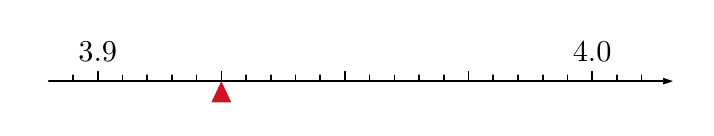
\begin{tikzpicture}[x=1bp,y=-1bp,line cap=round,line join=round]
  \path[use as bounding box] (0,0) rectangle (237,29);
  \clip (0,0) rectangle (237,29);
  \definecolor{diagramanswer}{RGB}{205,20,35}
  \draw[line width=.75bp] (7.6,19.25) -- (228.9,19.25);
  \fill (228.8,18.05) -- (232.3,19.25) -- (228.8,20.45) -- cycle;
  % The marks 3.9 and 4.0 enclose twenty intervals of length 0.005.
  \foreach \tick in {-1,...,22}{
    \pgfmathsetmacro\tickx{25.214+8.9*\tick}
    \pgfmathsetmacro\ticky{ifthenelse(mod(\tick,5)==0,15.8,17.1)}
    \draw[line width=.58bp] (\tickx,19.25) -- (\tickx,\ticky);
  }
  \node[anchor=base,inner sep=0pt,font=\fontsize{11.3bp}{12bp}\selectfont]
    at (25.214,12) {$3.9$};
  \node[anchor=base,inner sep=0pt,font=\fontsize{11.3bp}{12bp}\selectfont]
    at (203.214,12) {$4.0$};
  % 3.925 is the fifth subdivision to the right of 3.9.
  \fill[diagramanswer] (69.714,19.25) -- (66.143,26.857) --
    (73.286,26.857) -- cycle;
\end{tikzpicture}
